\documentclass[11pt,a4paper]{article}
\usepackage[margin=2.3cm]{geometry}
\usepackage{amsmath,amssymb,bm,graphicx,booktabs,xcolor,listings,hyperref,tikz,enumitem,caption,microtype}
\usepackage[numbers,sort&compress]{natbib}
\usepackage[section]{placeins}
\usetikzlibrary{positioning,arrows.meta}
\hypersetup{colorlinks=true,linkcolor=blue!50!black,citecolor=blue!50!black,urlcolor=blue!50!black}
\setlist{nosep}

% ---------- honesty macros -------------------------------------------------
% \todo   : something that must be filled in from a real run (never invent it)
% \verify : a statement about the original paper that must be checked against the PDF
\newcommand{\todo}[1]{\textcolor{red}{\textbf{[TODO: #1]}}}
\newcommand{\verify}[1]{\textcolor{orange!70!black}{\textbf{[VERIFY: #1]}}}
\newcommand{\resin}[1]{\IfFileExists{results/quantitative/#1}{\input{results/quantitative/#1}}{\todo{run the pipeline to generate \texttt{\detokenize{#1}}}}}
\newcommand{\figin}[2]{\IfFileExists{figures/#1.jpg}{\includegraphics[width=#2\linewidth]{figures/#1.jpg}}{\IfFileExists{figures/#1.png}{\includegraphics[width=#2\linewidth]{figures/#1.png}}{\fbox{\parbox{#2\linewidth}{\centering\todo{figure \texttt{\detokenize{#1}} not generated yet}\\[1.5em]}}}}}
\newcommand{\GC}{Grad-CAM}
\DeclareMathOperator{\ReLU}{ReLU}
\lstset{language=Python,basicstyle=\ttfamily\footnotesize,keywordstyle=\color{blue!60!black},commentstyle=\color{green!40!black},
        frame=single,breaklines=true,numbers=left,numberstyle=\tiny,xleftmargin=1.5em}

\title{\textbf{Grad-CAM: Visual Explanations for CNN Classifiers}\\[2mm]
\large Pattern Recognition (EE798R) --- Course Project}
\author{Aaradhya Rohi \quad (Roll no.\ 230011)}
\date{\today}

\begin{document}
\maketitle

\begin{abstract}
Deep convolutional networks classify images well but do not say \emph{where} in the image the evidence for a decision lies.
Gradient-weighted Class Activation Mapping (\GC)~\citep{selvaraju2017} answers this for almost any CNN by weighting the feature maps of a chosen convolutional layer with the spatially averaged gradient of the class score and keeping only positive evidence.
This report derives the method from first principles, shows that it reduces to Class Activation Mapping (CAM)~\citep{zhou2016} on a global-average-pooling classifier, and re-implements it from scratch in PyTorch.
We fine-tune an ImageNet-pretrained ResNet-50 on PASCAL VOC~2007 and measure how well the explanations localise objects, using ground-truth bounding boxes, against vanilla gradient saliency, CAM, Grad-CAM++ and a model-free centre prior.
We further study sensitivity to the target layer and to the binarisation threshold, the class-discriminativeness of the maps, runtime, and failure cases.
On the 7{,}013 image--class pairs of the VOC~2007 test set, \GC{} reaches 85.6\% pointing accuracy and 38.8\% box-localisation accuracy (IoU $\ge0.5$ at a threshold of 15\% of the map maximum), against 63.1\% and 23.1\% for a model-free centre prior; its pointing accuracy is statistically identical to CAM and Grad-CAM++, and its box advantage over them at the default threshold largely disappears when each method uses its own best threshold.
Deeper layers localise much better than shallow ones, \GC{} at the last stage costs about 2\% over a forward pass, and the main failures are small and very large objects, part-only responses, context cues and low classifier confidence.
\end{abstract}

\section{Introduction and Motivation}
A classifier that reports ``dog, 0.97'' is hard to trust or debug unless we can tell what it looked at.
Explanations are useful for (i) detecting shortcut learning, where the network relies on background or context instead of the object; (ii) understanding failures and misclassifications; (iii) building trust in safety-critical settings such as medical imaging; and (iv) scientific inspection of what a representation has learned.
The difficulty is that a CNN is a composition of millions of parameters, so a faithful, human-readable summary of ``where the evidence is'' must be computed, not read off.

Early gradient-based visualisations are sharp but noisy and tied to single pixels, while CAM is coarse but class-discriminative and requires a special architecture.
\GC{} was proposed to keep CAM's class-discriminative, region-level maps while removing the architectural restriction.
In this report we study \GC{} as a \emph{pattern-visualisation} tool and ask a concrete, measurable question: \textbf{when a CNN classifies a VOC image, how well does the \GC{} heat-map for a present class overlap the annotated object, and how does this compare with simpler explanation methods?}

\paragraph{Scope and contributions.}
(1) A self-contained derivation and interpretation of \GC{} (Sections~\ref{sec:theory}--\ref{sec:math}), including a proof that CAM is a special case. (2) An independent PyTorch implementation of \GC, vanilla saliency and CAM, with unit tests that check the CAM identity numerically (Section~\ref{sec:impl}). (3) A quantitative localisation study on the full VOC~2007 test set with confidence intervals, a threshold sweep, a layer ablation, a class-discrimination measure and timings (Sections~\ref{sec:setup}--\ref{sec:quant}). (4) A qualitative study with rule-based (not hand-picked) examples of success, partial, background-dependent, misclassification and multi-object cases (Section~\ref{sec:qual}). We do \emph{not} train anything at scale, and we do not claim to reproduce the ImageNet experiments of the original paper.

\paragraph{How results are labelled.}
Three kinds of statements appear: numbers \emph{reported by the original paper} (always marked as such and cited), numbers \emph{measured by us} (generated by the released scripts and read into the report from files), and \emph{expectations, hypotheses and interpretation} (explicitly worded as such, e.g.\ ``hypothesis'' or ``plausible reading'').

\section{Background and Related Work}
\subsection{Deep Neural Network Interpretability}
Interpretability methods for vision models fall into three families: \emph{backpropagation-based} methods that use gradients through the network (saliency, deconvolution, guided backpropagation, CAM-family methods), \emph{perturbation-based} methods that observe how the output changes when the input is altered (occlusion, LIME), and \emph{representation-space} visualisations that embed internal features in a low-dimensional space (t-SNE~\citep{vandermaaten2008}, UMAP~\citep{mcinnes2018}, Isomap~\citep{tenenbaum2000}, LLE~\citep{roweis2000}, MDS~\citep{kruskal1964}, Mapper~\citep{singh2007}).
The last family explains the \emph{geometry of a feature space} over many samples, not \emph{which pixels of one image} drove one prediction; it is therefore outside the scope of \GC{} and of this project (see Table~\ref{tab:syllabus}).

\subsection{Saliency Maps}
\textbf{Idea}: the pixels whose small change most affects the class score are important. \textbf{Mechanism}: \citet{simonyan2014} take $|\partial y^c/\partial \bm{x}|$ (maximum over colour channels) for input $\bm{x}$ and class score $y^c$. \textbf{Strength}: one backward pass, any differentiable model, pixel resolution. \textbf{Limitation}: the gradient is a \emph{local} linearisation of a highly non-linear function, so maps are noisy, scattered and do not form object-shaped regions.

\subsection{Deconvolution and Guided Backpropagation}
\citet{zeiler2014} and \citet{springenberg2015} also propagate a signal back to the image but modify the rule at ReLU units (pass only positive signals back; guided backpropagation additionally requires the forward activation to be positive).
\textbf{Strength}: visually sharp, edge-like detail. \textbf{Limitation}: the result is largely dependent on the input image rather than on the chosen class, and \citet{adebayo2018} report that some such methods are insensitive to the trained parameters, i.e.\ they behave partly like edge detectors. \GC{} was explicitly designed to supply the class-discriminative component these maps lack (the paper combines the two as Guided Grad-CAM; we do not study that combination).

\subsection{Class Activation Mapping}
\textbf{Idea}: if the last convolutional features are followed by global average pooling (GAP) and a single linear layer, then the class score is a weighted sum of spatially pooled feature maps, so the \emph{un}pooled weighted sum is a spatial evidence map. \textbf{Mechanism}: $M^c_{ij}=\sum_k w^c_k A^k_{ij}$ with $w^c_k$ the classifier weights~\citep{zhou2016}. \textbf{Strength}: class-discriminative, region-level, no gradients needed. \textbf{Limitation}: requires the GAP$\rightarrow$linear architecture; networks such as VGG-16 with fully connected layers must be modified and retrained.

\subsection{\GC{}}
\textbf{Idea}: replace CAM's classifier weights by gradient-derived channel importances. \textbf{Mechanism}: Eqs.~\eqref{eq:alpha}--\eqref{eq:cam} below. \textbf{Strength}: works for any CNN whose class score is differentiable with respect to a convolutional layer, with no retraining; the original paper also applies it to captioning, visual question answering and reinforcement-learning agents~\citep{selvaraju2017}. \textbf{Limitation}: coarse (resolution of the target layer), and the highlighted region is not guaranteed to be a causal explanation (Section~\ref{sec:limits}).


\begin{table}[t]\centering
\caption{CAM versus \GC. The last row is derived in Eq.~\eqref{eq:cam-special} and verified numerically in our tests; the other rows follow~\citep{zhou2016,selvaraju2017}.}\label{tab:camvsgc}
\small
\begin{tabular}{p{3.9cm}p{5.2cm}p{5.2cm}}
\toprule
Property & CAM & \GC \\ \midrule
Requires specific architecture? & Yes: last conv.\ layer $\rightarrow$ GAP $\rightarrow$ one linear layer & No: any CNN whose class score is differentiable w.r.t.\ a conv.\ layer \\
Requires GAP? & Yes & No \\
Requires classifier retraining/modification? & Yes, for networks not already of this form (e.g.\ replace FC layers by GAP + linear, retrain) & No: applied to the trained model as is \\
Uses gradients? & No: uses the classifier weights $w^c_k$ & Yes: weights $\alpha^c_k$ from gradients \\
Applicable to arbitrary CNN architectures? & No & Yes (also to non-classification heads, per the paper) \\
Spatial localisation & Coarse: resolution of the last conv.\ map & Coarse: resolution of the chosen layer (shallower layers give a finer grid) \\
Class-specific explanation? & Yes & Yes \\
Relation & -- & $=$ CAM up to a positive constant on a CAM-type network \\
\bottomrule
\end{tabular}
\end{table}

\subsection{Grad-CAM++, LIME and Other Related Methods}
Grad-CAM++~\citep{chattopadhay2018} keeps the form $\ReLU(\sum_k w_k A^k)$ but derives $w_k$ from higher-order gradient terms, so that several instances of an object or partially visible objects receive better coverage; it re-uses the same $A$ and gradients, so its cost equals \GC's. We use it as an extra comparison.
LIME~\citep{ribeiro2016} is model-agnostic: it perturbs superpixels of the image, queries the model many times and fits a sparse linear surrogate. It makes no use of the architecture, but costs hundreds of forward passes per image and depends on the segmentation and sampling; it is discussed here but \emph{not} implemented.

\begin{table}[t]\centering
\caption{Where each syllabus topic stands in this project. ``Core'' = used by \GC{} itself; ``Baseline'' = implemented and measured here; ``Related'' = discussed only.}\label{tab:syllabus}
\small
\begin{tabular}{p{4.4cm}p{2.3cm}p{7.5cm}}
\toprule
Topic & Role & Comment \\ \midrule
Backpropagation / gradient computation & Core & $\partial y^c/\partial A^k_{ij}$ is obtained by reverse-mode autodiff. \\
CNN feature representations & Core & Feature maps $A^k$ of the last convolutional stage. \\
\GC{} & Core & Re-implemented from scratch. \\
Saliency maps & Baseline & Vanilla gradient saliency. \\
CAM & Baseline & Exact for ResNet-50 (GAP + linear head). \\
Grad-CAM++ & Baseline (extra) & Closed-form variant on the same $A$, $G$. \\
LIME & Related & Perturbation-based, not implemented. \\
Guided backprop / deconvolution & Related & Not implemented; compared conceptually. \\
t-SNE, UMAP, Mapper, Isomap, LLE, MDS & Outside the paper & Feature-space visualisation, not used by \GC. \\
\bottomrule
\end{tabular}
\end{table}

\section{Theory and Conceptual Explanation}\label{sec:theory}
\subsection{CNN Feature Representations}
A convolutional stage applies a bank of $K$ learned filters to its input and a non-linearity, yielding $K$ feature maps $A^k\in\mathbb{R}^{h\times w}$. Because convolution and pooling are local and translation-equivariant, position $(i,j)$ of every map still corresponds to a definite (receptive-field) region of the image.
Early layers respond to edges and textures; deeper layers combine them into object parts and eventually category-specific patterns.

\subsection{Why Convolutional Feature Maps?}
A fully connected layer flattens the maps and destroys the spatial layout, so after it nothing says ``where''. The last convolutional layer is the deepest place where (a) the features are semantically rich and (b) spatial structure is still intact. Going deeper gives more semantics but a coarser grid; going shallower gives a finer grid but less class-specific content. This trade-off is the reason for the layer ablation in Section~\ref{sec:ablation}.

\subsection{Class-Specific Explanation}
For a fixed image different classes should give different maps. \GC{} achieves this because the weights $\alpha_k^c$ depend on the class $c$ through the gradient of that class's score, while the feature maps $A^k$ are shared. A channel that detects ``dog face'' receives a large positive weight for the class \emph{dog} and a small or negative one for \emph{cat}.

\subsection{\GC{} Intuition}
Each channel $A^k$ is a detector that says ``pattern $k$ occurs here''. The classifier then decides how much it cares about pattern $k$ for class $c$; that importance is $\alpha_k^c$. The heat-map is the sum of detectors weighted by importance: places where important patterns fire are hot.

\subsection{Complete Pipeline}
\begin{figure}[t]\centering
\resizebox{\linewidth}{!}{%
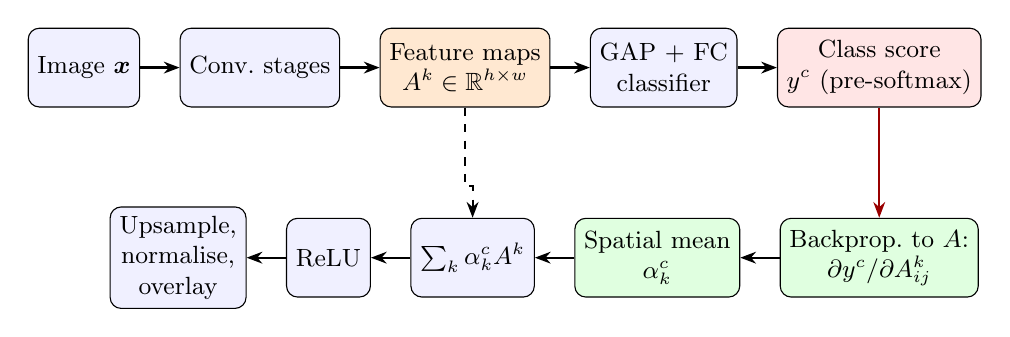
\begin{tikzpicture}[node distance=5mm, box/.style={draw, rounded corners, align=center, minimum height=10mm, font=\small, fill=blue!6},
  arr/.style={-{Stealth[length=2mm]}, thick}]
\node[box] (img) {Image $\bm{x}$};
\node[box, right=of img] (cnn) {Conv.\ stages};
\node[box, right=of cnn, fill=orange!18] (A) {Feature maps\\ $A^k\in\mathbb{R}^{h\times w}$};
\node[box, right=of A] (head) {GAP + FC\\ classifier};
\node[box, right=of head, fill=red!10] (y) {Class score\\ $y^c$ (pre-softmax)};
\draw[arr] (img)--(cnn); \draw[arr] (cnn)--(A); \draw[arr] (A)--(head); \draw[arr] (head)--(y);
\node[box, below=14mm of y, fill=green!12] (g) {Backprop.\ to $A$:\\ $\partial y^c/\partial A^k_{ij}$};
\node[box, left=of g, fill=green!12] (alpha) {Spatial mean\\ $\alpha_k^c$};
\node[box, left=of alpha] (sum) {$\sum_k \alpha_k^c A^k$};
\node[box, left=of sum] (relu) {ReLU};
\node[box, left=of relu] (up) {Upsample,\\ normalise,\\ overlay};
\draw[arr, red!60!black] (y)--(g); \draw[arr] (g)--(alpha); \draw[arr] (alpha)--(sum); \draw[arr] (sum)--(relu); \draw[arr] (relu)--(up);
\draw[arr, dashed] (A.south) |- ([yshift=4mm]sum.north) -- (sum.north);
\end{tikzpicture}}
\caption{The \GC{} pipeline. Top row: ordinary forward pass, the activations $A^k$ of the chosen layer are stored. Bottom row (right to left): the gradient of the class score is propagated back only as far as $A$, averaged over space to give the channel weights, combined with the stored maps, rectified, and resized to the image.}\label{fig:pipeline}
\end{figure}

\section{Mathematical Formulation}\label{sec:math}
\subsection{Target Class Score}
Let $\bm{x}$ be an image, $f$ the network, and $A^k\in\mathbb{R}^{h\times w}$ ($k=1,\dots,K$) the output of the chosen convolutional layer. Let $y^c$ denote the \emph{pre-softmax} score (logit) of class $c$. We use the logit rather than the softmax probability for a concrete reason: with $p_c=\mathrm{softmax}(y)_c$,
\begin{equation}
\frac{\partial p_c}{\partial A} = p_c\Big(\frac{\partial y^c}{\partial A}-\sum_j p_j \frac{\partial y^j}{\partial A}\Big),
\label{eq:softmax-grad}
\end{equation}
so the gradient of a probability mixes in all other classes and vanishes when $p_c\to1$ (saturation); the logit gradient isolates evidence for class $c$ alone. In our multi-label VOC model each logit feeds a sigmoid, and the same argument applies.

\subsection{Gradient Computation}
The quantity
\begin{equation}
g^{k}_{ij}=\frac{\partial y^c}{\partial A^k_{ij}}
\label{eq:grad}
\end{equation}
is the sensitivity of the class score to a unit change of the activation of channel $k$ at location $(i,j)$. It is obtained by one backward pass that starts at $y^c$ and stops at layer $A$ (reverse-mode differentiation, i.e.\ backpropagation). To first order, $y^c(A+\Delta)\approx y^c(A)+\sum_{k,i,j} g^{k}_{ij}\Delta^k_{ij}$, so $g^k_{ij}$ says how much increasing that single activation would raise the class score.

\subsection{Importance Weights}
Collapsing the spatial dimensions by averaging gives the channel weight
\begin{equation}
\alpha_k^c=\frac{1}{Z}\sum_{i}\sum_{j}\frac{\partial y^c}{\partial A^k_{ij}},\qquad Z=h\cdot w .
\label{eq:alpha}
\end{equation}
Here $Z$ is the number of spatial positions, $\alpha^c_k$ is the average marginal contribution of channel $k$ to class $c$, and the averaging is global average pooling of the gradient map. \emph{Why average?} A channel's pattern may occur anywhere; we want one number saying how useful the \emph{pattern} is, independent of position, and the mean is the natural linear aggregate: if the score were linear in the channel's total activation, $y^c\approx \sum_k \alpha_k^c \sum_{ij}A^k_{ij}$, then $\alpha_k^c$ is exactly its coefficient.

\paragraph{Proof that CAM is a special case.} Suppose the network ends in GAP followed by one linear layer with weights $w^c_k$ (bias omitted, as it does not depend on $A$): $y^c=\sum_k w^c_k\,\frac1Z\sum_{ij}A^k_{ij}$. Then $\partial y^c/\partial A^k_{ij}=w^c_k/Z$ for every $(i,j)$, hence
\begin{equation}
\alpha_k^c=\frac1Z\sum_{ij}\frac{w^c_k}{Z}=\frac{w^c_k}{Z},\qquad
L^c_{\text{\GC}}=\ReLU\Big(\sum_k\frac{w^c_k}{Z}A^k\Big)=\frac{1}{Z}\ReLU\big(M^c\big),
\label{eq:cam-special}
\end{equation}
where $M^c=\sum_k w^c_k A^k$ is the CAM map. So on a CAM-compatible network \GC{} equals CAM up to the constant $1/Z$ and a ReLU, which disappears after normalisation. The paper makes the same point; we additionally verify Eq.~\eqref{eq:cam-special} numerically in \texttt{tests/test\_gradcam.py} (Section~\ref{sec:impl}). ResNet-50 has exactly this structure after \texttt{layer4}, which is why it is a clean testbed for comparing the two.

\subsection{\GC{} Heat-map}
\begin{equation}
L^c_{\text{\GC}}=\ReLU\Big(\sum_{k=1}^{K}\alpha_k^c\,A^k\Big)\in\mathbb{R}^{h\times w}.
\label{eq:cam}
\end{equation}
\emph{Why a weighted sum of feature maps?} Each $A^k$ localises one pattern; the weighted sum is a spatial map of class-relevant pattern evidence, consistent with the linear model above. \emph{Why the final convolutional layer?} It is the deepest layer with intact spatial layout and the richest semantics (Section~\ref{sec:theory}); we test shallower layers in Section~\ref{sec:ablation}.

\subsection{ReLU and Upsampling}
\textbf{ReLU.} A negative contribution at $(i,j)$ means the pattern there \emph{lowers} the class score, which typically happens where evidence for \emph{other} classes lies. We want the region that supports class $c$, so negative values are clipped. The original paper reports that without the ReLU the maps tend to highlight more than the target class~\citep{selvaraju2017}. A consequence worth noting: if no location has positive net evidence, the map is identically zero. This does occur for classes the network does not believe are present; we count and report such \emph{empty maps} (Table~\ref{tab:main}).

\textbf{Upsampling and normalisation.} The map has the size $h\times w$ of the layer (e.g.\ $14\times14$ for \texttt{layer4} at $448\times448$ input). It is resized to image resolution by bilinear interpolation, $\tilde L^c=\mathrm{Resize}(L^c_{\text{\GC}})$, and min--max normalised to $[0,1]$ for display and thresholding. Bilinear interpolation produces a smooth map; it cannot add detail finer than the grid, which is the origin of \GC's coarse localisation.

\subsection{Interpretation of the Equations}
\begin{table}[h]\centering\caption{Symbols.}\small
\begin{tabular}{ll}\toprule
Symbol & Meaning \\ \midrule
$\bm x$, $c$ & input image, target class \\
$y^c$ & pre-softmax score of class $c$ \\
$A^k_{ij}$ & activation of channel $k$ at spatial location $(i,j)$ of the target layer \\
$K$, $h$, $w$, $Z=hw$ & number of channels, map height/width, number of positions \\
$\alpha_k^c$ & importance of channel $k$ for class $c$ (spatial mean of the gradient) \\
$L^c_{\text{\GC}}$ & coarse heat-map; $\tilde L^c$ its upsampled, normalised version \\ \bottomrule
\end{tabular}\end{table}
The chain \emph{CNN representation} $\rightarrow$ \emph{gradient-based channel importance} $\rightarrow$ \emph{weighted feature maps} $\rightarrow$ \emph{ReLU} $\rightarrow$ \emph{heat-map} corresponds to Eqs.~\eqref{eq:grad}, \eqref{eq:alpha}, \eqref{eq:cam} and the resize step.
\paragraph{Complexity.} The forward pass costs $O(F)$ ($F$ = network FLOPs). The backward pass runs only from the logits to the target layer, so for the last stage of ResNet-50 it covers just the average-pool and the linear layer: negligible next to $F$. Shallower targets need back-propagation through the stages above them. The map itself costs $O(Khw)$ and the resize $O(HW)$. Memory: the stored activations $K\cdot h\cdot w$ floats (for \texttt{layer4}, $2048\times14\times14\approx0.4$M floats). These are theoretical statements; measured times are in Section~\ref{sec:compute}.

\section{Algorithm / Methodology}
\subsection{Input}
Image $\bm x\in\mathbb{R}^{3\times H\times W}$ (ImageNet-normalised), a trained network, a target layer, and a class index $c$ (not necessarily the predicted one). \textbf{Output}: a heat-map $\tilde L^c\in[0,1]^{H\times W}$.
\subsection{Forward Pass}
Run the network; a forward hook stores $A$ of the target layer without detaching it from the graph.
\subsection{Backward Pass}
Differentiate the scalar $y^c$ with respect to $A$ (not the parameters) to obtain $G=\partial y^c/\partial A$.
\subsection{Heatmap Construction}
Compute $\alpha$ by averaging $G$ over space, form $\ReLU(\sum_k\alpha_kA^k)$, resize, and normalise.
\subsection{Visualisation and Localisation}
For display the map is colour-coded and blended with the image. For \emph{evaluation} the map is converted into a region by the protocol below (Section~\ref{sec:metrics}).

\begin{figure}[h]\centering
\fbox{\begin{minipage}{0.92\linewidth}\small
\textbf{Algorithm 1} \GC{} for image $\bm x$, class $c$, layer $\ell$\\
1.\ $y\leftarrow f(\bm x)$; store $A\leftarrow$ output of layer $\ell$\\
2.\ $G\leftarrow\partial y^c/\partial A$ \hfill (one partial backward pass)\\
3.\ $\alpha_k\leftarrow\frac1Z\sum_{ij}G^k_{ij}$ for $k=1..K$\\
4.\ $L\leftarrow\ReLU(\sum_k\alpha_kA^k)$\\
5.\ $\tilde L\leftarrow\mathrm{Resize}(L,(H,W))$; $\tilde L\leftarrow(\tilde L-\min\tilde L)/(\max\tilde L-\min\tilde L+\epsilon)$\\
6.\ \textbf{return} $\tilde L$
\end{minipage}}
\caption{Pseudocode of the method as implemented in \texttt{src/gradcam.py}.}
\end{figure}

\section{Implementation}\label{sec:impl}
\subsection{Framework and Environment}
PyTorch~\citep{paszke2019} with torchvision. \textbf{Libraries used}: PyTorch/torchvision (autodiff, ResNet-50 definition and ImageNet weights, \texttt{VOCDetection} file parsing), SciPy~\citep{virtanen2020} (connected components), scikit-learn~\citep{pedregosa2011} (average precision), NumPy/pandas/Matplotlib. \textbf{Written for this project}: all explanation methods (\texttt{gradcam.py}, \texttt{saliency.py}, \texttt{cam.py}), the dataset wrapper, the localisation metrics, the evaluation/benchmark/figure scripts and the unit tests. No existing \GC{} repository or package (e.g.\ \texttt{pytorch-grad-cam}) was used or consulted for the code. I ran all the experiments on Colab, and the results and conclusions come from those runs.
\subsection{Model}
ResNet-50~\citep{he2016} with ImageNet-pretrained weights~\citep{russakovsky2015}. We chose it because (i) it is small enough for a free Colab GPU, (ii) after \texttt{layer4} it has exactly the GAP$\rightarrow$linear structure so that CAM is applicable and the baseline comparison is exact, and (iii) it has three natural stages (\texttt{layer2/3/4}, strides 8/16/32) for the layer ablation. VGG-16 was the original paper's main network but needs a modified, retrained head for CAM. The 1000-way head is replaced by a 20-way linear layer (multi-label, sigmoid).
\subsection{Dataset Processing}
Described in Section~\ref{sec:setup}. Images are resized to $448\times448$ so that \texttt{layer4} yields a $14\times14$ map ($7\times7$ at the usual $224$ input would be very coarse); boxes are rescaled accordingly.
\subsection{\GC{} Implementation}
\textbf{Capturing activations.} A forward hook stores the layer output \emph{with its graph}:
\lstinputlisting{snippets/hook.py}
\textbf{Gradients of the class score.} We differentiate the logit with respect to the stored activations only; no parameter gradients are computed:
\lstinputlisting{snippets/backward.py}
\textbf{Weights, weighted sum, ReLU} --- Eqs.~\eqref{eq:alpha} and~\eqref{eq:cam}:
\lstinputlisting{snippets/core.py}
Lines~1 and~2 correspond one-to-one to Eqs.~\eqref{eq:alpha} and~\eqref{eq:cam}; \texttt{G.mean(dim=(2,3))} is the spatial average and the broadcasted product followed by \texttt{sum(dim=1)} is the weighted sum over channels. The result is resized bilinearly and min--max normalised (\texttt{upsample}, \texttt{normalize\_map}). \textbf{Verification.} \texttt{tests/test\_gradcam.py} checks (a) Eq.~\eqref{eq:cam-special} numerically on ResNet-50 ($\alpha=w/Z$ and map $=\ReLU(M^c)/Z$), (b) that our \texttt{autograd.grad} route gives the same $\alpha$ as an independent \texttt{backward()}+\texttt{retain\_grad()} route at \texttt{layer2/3/4}, (c) output range and class-specificity, and (d) the IoU/box code. These tests use random weights and synthetic inputs; they validate the code and produce no experimental results.
\subsection{Baseline Implementation}
\textbf{Vanilla saliency} (\texttt{saliency.py}) differentiates the same logit with respect to the \emph{input}:
\lstinputlisting{snippets/saliency.py}
\textbf{CAM} (\texttt{cam.py}) uses the weights of the final linear layer: $M^c_{ij}=\sum_kw^c_kA^k_{ij}$, min--max normalised without ReLU, as in~\citep{zhou2016}. \textbf{Grad-CAM++} (\texttt{gradcam.py}) re-uses $A$ and $G$ with the closed-form weights of~\citep{chattopadhay2018}. \textbf{Centre Gaussian}: a model-free, isotropic Gaussian ($\sigma=0.25\times$ image size) --- a sanity control that exposes how much of the localisation score is explained by objects simply being near the middle of VOC images.

\section{Dataset and Experimental Setup}\label{sec:setup}
\subsection{Dataset}
PASCAL VOC~2007~\citep{everingham2010,voc2007}: 20 object categories, images with bounding-box annotations and a \emph{difficult} flag; 5{,}011 \texttt{trainval} and 4{,}952 \texttt{test} images. It is publicly downloadable, annotated with boxes (needed for our metric), and was also used by the original paper's community for weakly-supervised tasks. The images were collected from Flickr; usage terms are given on the dataset website~\citep{voc2007}. Image-level labels are derived from the boxes; \emph{difficult} objects are ignored for both labels and boxes.
\subsection{Train/Validation/Test Split}
\texttt{trainval} is split 90\%/10\% (seeded) into training and validation (used only to pick the checkpoint by mAP); the \texttt{test} split is used only for evaluation. Exact counts are listed in Section~\ref{sec:hw}.
\subsection{Preprocessing}
Anisotropic resize to $448\times448$ (bicubic), ImageNet mean/std normalisation; random horizontal flip during training only.
\subsection{Model Configuration and Hyper-parameters}
Only \texttt{layer4} and the new head are trained; earlier stages and their batch-norm statistics stay frozen. Binary cross-entropy on logits, AdamW~\citep{loshchilov2019}, learning rates $10^{-3}$ (head) and $10^{-4}$ (\texttt{layer4}), weight decay $10^{-4}$, cosine schedule, batch size 32, 6 epochs, seed 0, mixed precision on GPU (the defaults of \texttt{scripts/train.py}, which were used unchanged; they are recorded in \texttt{train\_log.json}). The explanation experiments do not train anything further.
\subsection{Evaluation Metrics}\label{sec:metrics}
We evaluate the explanation for each ground-truth \emph{(image, class)} pair, using the ground-truth class (not the prediction), so that all methods are scored on identical pairs. For a map $\tilde L\in[0,1]^{H\times W}$ and the set $\mathcal{B}_c$ of non-difficult boxes of class $c$:
\begin{enumerate}
\item \textbf{Localisation accuracy.} Binarise $\tilde L\ge\tau$ (default $\tau=0.15$ of the maximum, following the weakly-supervised localisation protocol of the original paper~(Section~4.1 of the paper: threshold at 15\% of the maximum, box around the single largest segment)), keep the largest 4-connected component, take its bounding box $B_{\text{pred}}$, and compute
$\mathrm{IoU}=|B_{\text{pred}}\cap B|/|B_{\text{pred}}\cup B|$ against each $B\in\mathcal{B}_c$; the pair counts as correct if $\max_B\mathrm{IoU}\ge0.5$ (the best match is used because several instances of a class may exist). An empty map has IoU $=0$.
\item \textbf{Mean IoU} (same quantity, averaged).
\item \textbf{Pointing game}~\citep{zhang2018}: correct if the maximum of $\tilde L$ lies inside some box of $\mathcal{B}_c$ (no tolerance; empty maps are failures).
\item \textbf{Mass in GT}: $\sum_{p\in\cup\mathcal{B}_c}\tilde L(p)\big/\sum_p\tilde L(p)$, a threshold-free measure of how much of the map's energy lies on the object.
\item \textbf{Class-discrimination index}: on images with $\ge2$ classes, for classes $c\neq c'$ the mean map value on pixels covered only by $c$'s boxes divided by the sum of that and the mean value on pixels covered only by $c'$'s boxes (0.5 = cannot tell the classes apart).
\item \textbf{Cost}: wall-clock per explanation, peak GPU memory, parameter count.
\end{enumerate}
Uncertainty: 95\% percentile bootstrap intervals~\citep{efron1979} over pairs; differences between methods use a \emph{paired} bootstrap because all methods are scored on the same pairs.
\paragraph{Why these metrics.} IoU and localisation accuracy answer ``does the highlighted region match the object?'' but depend on the threshold and on box shape; the pointing game and mass are insensitive to the threshold; the discrimination index probes the claim that \GC{} is class-specific. None of them measures \emph{faithfulness} to the model (deletion/insertion), which we list as a limitation.
\subsection{Hardware, Software and Run Facts}\label{sec:hw}
\resin{setup_facts.tex}

\section{Quantitative Results}\label{sec:quant}
All numbers in this section were measured in this project (VOC2007 test, all 4{,}952 images, 7{,}013 image--class pairs, one run, seed 0) and are read from the files written by \texttt{evaluate.py}, \texttt{benchmark.py}, \texttt{make\_tables.py} and \texttt{extra\_analysis.py}; none is taken from the original paper. The fine-tuned classifier reaches a test mAP of 0.918 (Section~\ref{sec:hw}), so most ground-truth classes are recognised and the explanations are of a competent model.
\resin{main_table.tex}
\paragraph{Reading Table~\ref{tab:main}.} At the default threshold $\tau=0.15$ \GC{} localises best: 38.8\% of the pairs reach IoU $\ge0.5$ (95\% CI 37.7--40.0), against 33.0\% for Grad-CAM++, 28.3\% for CAM, 23.1\% for the model-free centre Gaussian and 0.6\% for vanilla saliency; mean IoU follows the same order (0.423, 0.379, 0.348, 0.304, 0.038). The paired bootstrap (Table~\ref{tab:paired}) excludes zero for every localisation-accuracy comparison: \GC{} is 5.8 points above Grad-CAM++ (CI $+4.9$ to $+6.9$), 10.6 above CAM (CI $+9.5$ to $+11.6$) and 15.7 above the centre prior. The pointing game tells a different story: \GC{} (85.6\%), Grad-CAM++ (85.9\%) and CAM (85.6\%) are statistically indistinguishable (paired differences $-0.3$ [$-0.8,+0.2$] and $-0.0$), and all are about 22 points above the centre control (63.1\%). \GC{} and CAM disagree on exactly one of 7{,}013 pairs, and in that pair the \GC{} map has zero energy inside the ground-truth boxes (\texttt{extra.json}). This is what Eq.~\eqref{eq:cam-special} predicts: the two maps have the same arg-max wherever \GC{} is non-empty.
\resin{paired_table.tex}
\paragraph{Why do the box metrics separate methods that point to the same place?} The answer is in the size of the predicted box (Table~\ref{tab:boxarea}). At $\tau=0.15$ the CAM box has a median area of 94.4\% of the image and exceeds 90\% of the image in 52.7\% of the pairs, almost like the centre prior (median 94.7\%), whereas the \GC{} box has a median of 39.9\%. Our CAM is min--max normalised without a ReLU (as in the CAM paper), so its zero level sits above 0 after normalisation and a 15\% threshold admits most of the image; \GC{} clips negative evidence to 0 first, so 15\% of its maximum is a much tighter region. Two observations are consistent with this reading: the CAM and Grad-CAM++ accuracy curves peak at higher thresholds ($\tau=0.3$) than \GC's ($\tau=0.2$; Table~\ref{tab:thr}), and CAM's share of heat-map energy inside the ground-truth boxes (48.2\%) is lower than \GC's (64.1\%). We did not run a separate control that changes only the normalisation, so this is a well-supported explanation rather than an isolated test. Conversely, vanilla saliency produces extremely peaked maps: its box at $\tau=0.15$ covers on average 0.4\% of the image, hence IoU $\approx0$ and 0.6\% accuracy. This number reflects our simple protocol (threshold plus largest component, no smoothing or grab-cut as in the baseline of the original paper), not an intrinsic uselessness of gradient saliency; its pointing accuracy of 68.5\% [67.5, 69.7] is above the centre control (63.1\%) but only by 5 points.
\resin{boxarea_table.tex}
\paragraph{Centre control.} A Gaussian that ignores the image already reaches 23.1\% localisation and 63.1\% pointing accuracy, because VOC objects are large (median ground-truth region 27\% of the image, mean 33\%) and often centred. Any claim of a method's quality must therefore be read relative to this control, not relative to zero; in particular, Section~\ref{sec:failures} shows that for objects covering more than 60\% of the image the centre control beats \GC.
\paragraph{Empty maps.} \GC{} returned an identically zero map for 0.2\% of the pairs (16 pairs); Grad-CAM++ and CAM never did. A further set of pairs have a non-empty map with exactly zero energy inside the object boxes (69 \GC{} pairs in total with zero mass, all with classifier probability for the class below 0.13; Table~\ref{tab:conf}).
\resin{discrimination_table.tex}
\paragraph{Class discrimination.} On the 3{,}644 ordered class pairs from images with at least two annotated classes, the \GC{} map of class $c$ puts clearly more heat on pixels that belong only to $c$ than on pixels that belong only to the other class (index 0.850, CI 0.844--0.856). The centre Gaussian scores 0.500 [0.494, 0.506], which validates the index (a map with no class information is at chance). CAM reaches 0.731, vanilla saliency 0.664 and Grad-CAM++ 0.658. Since our CAM differs from \GC{} only by the ReLU (and the resulting zero-anchored normalisation), the 12-point gap quantifies what the rectification removes, in the direction the original paper describes (negative evidence belongs to other classes; Section~3 of~\citep{selvaraju2017}). This is an automatic proxy based on box overlap, not the human class-discrimination study of the paper.
\paragraph{Expectation stated before measuring, and the outcome.} We expected (i) \GC{} and CAM to be close on ResNet-50 because of Eq.~\eqref{eq:cam-special}, (ii) saliency to score lowest on box-IoU, and (iii) high-resolution maps to do relatively better on pointing than on box-IoU. (ii) was confirmed. (i) was only partly right: the arg-max (pointing) is identical, but the thresholded metrics differ by 10.6 points because normalisation changes which region survives the threshold, so ``close'' holds for \emph{where} the evidence peaks and not for the \emph{extent} of the box. (iii) holds for saliency (68.5\% pointing against 0.6\% box accuracy).

\section{Qualitative Results}\label{sec:qual}
Examples are chosen by fixed rules with a fixed random seed (\texttt{scripts/generate\_heatmaps.py}), not by hand; the rules and the number of pairs that satisfy them are in the captions. Each row shows the image with the ground-truth boxes of the explained class (green; other classes yellow), the \GC{} heat-map, the overlay with the predicted box (red), and Grad-CAM++, CAM and vanilla saliency. Descriptions below are of what is visible in these specific rows; they illustrate patterns and do not by themselves prove them (the quantitative tables do).
\begin{figure}[!t]\centering\figin{fig_success}{0.98}
\caption{\emph{Successful explanations}: random sample from the 2{,}624 pairs (37.4\%) with IoU $\ge0.5$ and a pointing hit at $\tau=0.15$. Rows: bicycle, dog, train, chair.}\label{fig:success}\end{figure}
\paragraph{Successes (Figure~\ref{fig:success}).} In the bicycle and dog rows the hot region covers the object body (frame and wheels; head and chest) and little of the surroundings; in the train row the strongest response is at the front end of the train with a weaker band along the carriage, and the red box also spills below onto the track and to the right (it still passes the IoU test); in the chair row the peak is on the seat and legs of the chair (classifier probability 0.49) but a second weaker region appears at the right edge. Grad-CAM++ and CAM overlays are visually very similar to each other and broader than \GC's, in line with their larger boxes (Table~\ref{tab:boxarea}). Saliency is a diffuse speckle within and around the object that cannot be turned into a region by a threshold.
\begin{figure}[!t]\centering\figin{fig_partial}{0.98}
\caption{\emph{Partial explanations}: random sample from the 375 pairs (5.3\%) with a pointing hit but a predicted box smaller than half of the ground-truth area. Rows: person, chair, dog, potted plant.}\label{fig:partial}\end{figure}
\paragraph{Partial explanations (Figure~\ref{fig:partial}).} The hot region sits on the most characteristic part: the cyclist's helmet and upper body (person), the face of the dog, and the pot (soil and rim) rather than the foliage of the potted plant; for the chair (probability 0.02) only a small spot near the seat survives while the CAM overlay is diffusely warm over the whole picture. The ground-truth boxes cover the entire object (or nearly the entire image), so these boxes score poorly even though the model is plausibly attending to the right object part.
\begin{figure}[!t]\centering\figin{fig_background}{0.98}
\caption{\emph{Background / context dependence}: random sample from the 559 pairs (8.0\%) with a pointing miss and less than 30\% of the map's energy inside the ground-truth boxes. Rows: bottle, chair, bottle, chair.}\label{fig:background}\end{figure}
\paragraph{Background and context (Figure~\ref{fig:background}).} The first bottle (probability 0.02) has its hot spot next to, not inside, the annotated object. In the second row the strongest regions are the lower-left corner (a small white step stool) and the right edge of the armchair rather than the annotated armchair body; in the third row the heat covers the dinner-table scene with plates and food around the thin bottle boxes; in the last row the legs of a large black table and a sofa light up while the annotated chair is a small object far behind. A plausible reading is that the model uses co-occurring context or look-alike furniture (a stool for a chair, a dinner table for bottles); we did not test this with interventions, so it remains a hypothesis.
\begin{figure}[!t]\centering\figin{fig_misclassification}{0.98}
\caption{\emph{Misclassification}: random sample of images whose top-1 predicted class is absent from the ground truth; the maps explain the \emph{predicted} class (probability in the row label). Rows: potted plant, person, chair, tv monitor.}\label{fig:mis}\end{figure}
\paragraph{Misclassification (Figure~\ref{fig:mis}).} The explanation often makes the error understandable: for ``potted plant'' (0.10) the peak is on the greenery behind the pool; for ``person'' (0.45) it is on bare feet and legs; for ``tv monitor'' (1.00) it is on the television screen, which visibly shows a person. The last row is probably not a model error at all: the television is present but not counted as a ground-truth class, likely because VOC marks it \emph{difficult} and our labels ignore difficult objects (not checked in the annotation file). Our ``top-1 not in ground truth'' rule therefore also catches annotation artefacts and low-confidence images (the top class has probability only 0.10 in the first row).
\begin{figure}[!t]\centering\figin{fig_multiobject}{0.98}
\caption{\emph{Several classes in one image}: two images, each explained for two of its classes in consecutive rows (motorbike and person in both).}\label{fig:multi}\end{figure}
\paragraph{Multiple classes (Figure~\ref{fig:multi}).} In the first image the motorbike map is concentrated on the lower and central part of the bike while the person map is on the upper right where the people's heads and torsos are; in the second image the motorbike map is scattered over several regions (left edge, handlebar area, rear wheel) while the person map is a single horizontal band around the small distant figure. The maps for the two classes are clearly different, as the discrimination index (Table~\ref{tab:disc}) suggests quantitatively; they are not perfect (the motorbike map in the second image is fragmented).

\section{Analysis and Discussion}
\subsection{Comparison with Baseline}
\GC{} is the best of the five methods on every box-based metric at the default threshold, but the margin has three different sources that should not be confused. (1) \emph{Against saliency} the difference is large and real for pointing too (+17.1 points, CI $+15.9$ to $+18.2$): a one-step gradient with respect to pixels is local and noisy, whereas \GC{} aggregates a semantically rich layer; the box-metric gap (+38.2) is exaggerated by our naive region extraction. (2) \emph{Against CAM} the pointing result is identical, as the derivation predicts, and the box gap (+10.6) is explained by the ReLU and zero-anchored normalisation, which shrink \GC's region, not by better evidence. (3) \emph{Against Grad-CAM++} the pointing difference is not significant either, and the box gap (+5.8) again comes mainly from region size at a fixed $\tau$. When each method is allowed its own best threshold (Table~\ref{tab:thr}) the three CAM-family methods reach 39.4\% (\GC, $\tau=0.2$, CI 38.4--40.5), 39.7\% (Grad-CAM++, $\tau=0.3$, CI 38.5--40.7) and 38.3\% (CAM, $\tau=0.3$, CI 37.2--39.4), whose confidence intervals overlap almost entirely. Because these thresholds were picked on the test set the values are optimistic and no paired test was run at the best thresholds, so the safe conclusion is: \emph{we see no evidence that one of the three gives better object extents than the others once the threshold is calibrated; \GC's advantage at $\tau=0.15$ is mostly a calibration effect}. The advantage over the centre control (+15.7 points localisation, +22.5 pointing) is genuine, but it is concentrated in small and medium objects (Table~\ref{tab:size}).
\subsection{Successful Examples}
In the 2{,}624 successes (37.4\% of pairs; Figure~\ref{fig:success}) the classifier is confident and the object is mid-sized to large. Success rises steeply with classifier confidence (44.5\% localisation accuracy when the class probability is $\ge0.9$, Table~\ref{tab:conf}) and with object size. Per class (Table~\ref{tab:class}) \GC{} does best on cat (63.0\%), sofa (57.8\%), dog and dining table (57.4\%) and horse (56.6\%): compact, large, distinctive objects.
\subsection{Failure Cases}\label{sec:failures}
We distinguish observed facts (from tables and figures) from hypotheses.
\begin{enumerate}[leftmargin=*]
\item \textbf{Small objects and the coarse grid.} For objects covering less than 10\% of the image, \GC{} reaches 3.9\% localisation accuracy but 67.8\% pointing accuracy, far above the centre control's 18.2\% (Table~\ref{tab:size}). The predicted box is on average 21.0\% of the image for objects whose ground truth is 4.5\% (measured), i.e.\ it finds the object but the region is several times too large. \emph{Hypothesis}: with a $14\times14$ grid at layer4 one cell is about 0.5\% of the image and bilinear upsampling spreads each activation over its neighbours, so small objects cannot be delineated; layer3 (28$\times$28) was nevertheless worse overall (Section~\ref{sec:ablation}), so resolution alone does not fix it.
\item \textbf{Large objects: the box under-fills, and a no-model prior wins.} For objects covering more than 60\% of the image the \GC{} box averages 67.6\% of the image versus a ground truth of 76.5\%, and localisation accuracy is 67.7\% against 84.1\% for the centre prior, 83.9\% for CAM and 84.2\% for Grad-CAM++ (Table~\ref{tab:size}). Methods that output a near-full-image box win here by construction. The overall ranking is thus partly a statement about the size mix of VOC, which is a limitation of box-IoU as a metric.
\item \textbf{Pointing is right, region is wrong.} In 3{,}381 pairs (48.2\%) the \GC{} peak lies inside a ground-truth box but IoU is below 0.5. This is the dominant failure of the box metric and combines patterns~1 and~2 with partial coverage of the object (Figure~\ref{fig:partial}: the helmet, the dog's face and the pot are discriminative parts; 375 pairs, 5.3\%, satisfy the strict ``box under half the ground truth'' rule). \emph{Hypothesis}: the classifier relies on the most discriminative part, and the gradient weights follow that part.
\item \textbf{The classifier does not recognise the class.} Localisation accuracy falls from 44.5\% (probability $\ge0.9$) to 30.9\% (0.5--0.9), 21.9\% (0.1--0.5) and 11.5\% ($<0.1$); pointing falls from 89.7\% to 56.5\% (Table~\ref{tab:conf}). 1{,}084 of the 7{,}013 pairs have probability below 0.5. Of the 69 pairs with zero mass inside the object, 68 are in the lowest bin. Mechanistically, \GC{} reports the evidence the network \emph{has} for the class; when the network sees no evidence the map is empty (16 pairs) or points elsewhere, which is the correct behaviour for an explanation but counts as a failure for an object-localisation metric.
\item \textbf{Context and look-alikes.} 559 pairs (8.0\%) are pointing misses with little energy on the object (Figure~\ref{fig:background}); chair, bottle and tv monitor have the lowest accuracy (10.6\%, 11.3\%, 14.0\%; Table~\ref{tab:class}), and also the smallest ground-truth regions (22\%, 12\%, 17\% of the image on average), so size and context are confounded. \emph{Hypothesis} from the figures: furniture and dinner-table context drive these classes; we did not run an occlusion or counterfactual test to separate context from size.
\item \textbf{Multiple instances (hypothesis only).} Person has 2{,}007 pairs (29\% of all) and 30.3\% accuracy. We extract a single connected component as the box, while the best-IoU is taken over instances; a map covering several people therefore yields one merged or one partial box. We did not measure this directly.
\item \textbf{Does the target class change the map? Yes.} In Figure~\ref{fig:multi} the same image gives visibly different maps for motorbike and person, and the discrimination index is 0.850 against 0.500 for a class-blind map.
\end{enumerate}
\resin{size_table.tex}
\resin{confidence_table.tex}
\resin{class_table.tex}
\subsection{Sensitivity / Ablation Analysis}\label{sec:ablation}
Two analyses were performed: the target layer (\texttt{layer2/3/4}) and the binarisation threshold. An input-perturbation study (occlusion, noise) was not performed.
\resin{layer_table.tex}
\paragraph{Target layer.} Localisation accuracy increases monotonically with depth, from 12.1\% (layer2, $56\times56$ map) through 29.5\% (layer3, $28\times28$) to 38.8\% (layer4, $14\times14$); pointing rises from 50.6\% to 72.9\% to 85.6\%, and the share of energy on the object from 36.9\% to 44.7\% to 64.1\%. Layer4 is significantly better than both shallower layers in the paired test (Table~\ref{tab:paired}; layer4 minus layer2: $+26.7$ [$+25.5,+27.8$], minus layer3: $+9.3$ [$+8.2,+10.5$]). Layer2 is \emph{below} the model-free centre control on pointing (50.6\% vs.\ 63.1\%) and on energy on the object (36.9\% vs.\ 43.7\%): its maps carry little class-specific information. Figure~\ref{fig:layers} shows why: at layer2 the map is a speckle over background texture such as the grass around the dog, at layer3 object parts (wheels, dog face) appear alongside many background spots, and layer4 gives a compact blob on the object. So finer resolution does not compensate for weaker semantics, in agreement with the trade-off argued in Section~\ref{sec:theory} and with the statement of the original paper that the discriminative ability of \GC{} reduces going to shallower layers of ResNets~\citep{selvaraju2017}. (We measured this on classification localisation; the paper's statement concerns a different visualisation.)
\begin{figure}[t]\centering\figin{fig_layers}{0.75}\caption{\GC{} at \texttt{layer2}, \texttt{layer3} and \texttt{layer4} for the four successful pairs of Figure~\ref{fig:success} (bicycle, dog, train, chair). Resolution increases toward the left, semantic specificity toward the right.}\label{fig:layers}\end{figure}
\resin{threshold_table.tex}
\begin{figure}[t]\centering\figin{threshold_sweep}{0.6}\caption{Localisation accuracy as a function of the threshold $\tau$ for each method (measured, VOC2007 test).}\label{fig:thr}\end{figure}
\paragraph{Threshold.} The optimum depends strongly on the method: \GC{} peaks at $\tau=0.2$ (39.4\%) and is fairly flat between 0.1 and 0.3 (37.1--39.4\%); CAM and Grad-CAM++ peak at $\tau=0.3$ (38.3\% and 39.7\%) and are much worse at 0.05--0.15; the centre control also peaks at 0.3 (29.1\%); saliency is best at the smallest threshold (15.2\% at 0.05) and collapses afterwards. The ranking of the methods therefore changes with $\tau$: \GC{} leads at $\tau\le0.2$; from $\tau=0.3$ on Grad-CAM++ and CAM are ahead of it (at $\tau=0.3$: 39.7\% and 38.3\% against 37.1\%; at $\tau=0.5$: 31.8\% and 33.6\% against 24.6\%). Any statement ``method A localises better than B'' based on a single threshold should be treated with caution.
\subsection{Computational Analysis}\label{sec:compute}
\resin{timing_table.tex}
Measured on a Tesla T4 at $448\times448$, batch size 1, full precision, 100 timed runs after warm-up: \GC{} at layer4 costs 19.2 ms against 18.8 ms for the plain forward pass (+0.4 ms, about 2\%), because the backward pass starts at the logit and stops at the layer4 output, crossing only the pooling and the linear layer. Targeting layer2 requires back-propagating through layer3 and layer4 and costs 32.0 ms (+70\%). Grad-CAM++ adds about 0.8 ms to \GC{}, CAM needs 19.7 ms, and vanilla saliency, which back-propagates to the input, needs 69.2 ms (3.7 times the forward pass). The model has 23{,}549{,}012 parameters. Peak GPU memory is 243 MB for a forward pass but 705 MB for \GC{} at layer4 (788 MB at layer2) and only 257 MB for CAM. This is higher than the theoretical activation storage ($K\cdot h\cdot w\approx0.4$M floats) discussed in Section~\ref{sec:math}; \emph{hypothesis}: because our implementation lets autograd record the whole forward pass (it makes the input require gradients), intermediate activations are kept. A variant that differentiates only the last stage from a detached activation would likely need less memory; we did not test it. FLOPs were not measured. In practice \GC{} at the last stage is almost free relative to inference, which is a strong deployment argument over perturbation methods such as LIME that need hundreds of forward passes (not measured here).
\subsection{Limitations}\label{sec:limits}
\textbf{From the literature.} (i) The map has the grid size of the target layer, so fine boundaries and small objects are poorly delineated. (ii) A highlighted region is not proof that the model \emph{used} it: \citet{adebayo2018} urge sanity checks for saliency methods, and \citet{draelos2020} propose HiResCAM because, they argue, the spatial averaging of gradients can make the map unfaithful to the model's actual computation in some architectures. (iii) Results depend on the chosen layer. (iv) The explanation reflects the classifier's evidence, which may be wrong. \textbf{Observed here.} (a) Localisation scores depend heavily on the threshold and on normalisation (Tables~\ref{tab:thr},\ref{tab:boxarea}); (b) box-IoU is confounded by object size and VOC's centre bias, since a model-free Gaussian scores 23.1\% and beats \GC{} on objects covering more than 60\% of the image; (c) low-confidence classes yield empty or off-object maps; (d) the coarse $14\times14$ map is too large for small objects. \textbf{Limits of our protocol.} One architecture and dataset, one training run and seed, boxes instead of masks, no deletion/insertion or occlusion faithfulness test, no human study, thresholds for the best-case comparison chosen on the test set, saliency scored with a deliberately simple region extraction, and a misclassification rule that also catches annotation artefacts.

\subsection{Comparison with the Original Paper}
\textbf{Original-paper results (Table~1 and Section~4.1 of~\citep{selvaraju2017}).} The authors evaluate weakly-supervised localisation on the ILSVRC-15 validation set with an off-the-shelf VGG-16: they generate maps for the predicted classes, binarise at 15\% of the maximum, and draw a box around the single largest connected segment; localisation error is reported for the top-1 and top-5 predicted categories. We use the same 15\% threshold and largest-component rule, but everything else differs.
\begin{table}[h]\centering\caption{Original-paper numbers versus ours. Left block: values \emph{copied from Table~1 of the paper} (localisation \emph{error} in \%, lower is better). Right block: \emph{our measurements} (localisation \emph{accuracy} in \%, higher is better). The two blocks use different datasets, networks and metrics and must not be compared numerically.}\small
\resizebox{\linewidth}{!}{%
\begin{tabular}{lcc|cc}\toprule
 & \multicolumn{2}{c|}{Paper: ILSVRC-15 val, VGG-16} & \multicolumn{2}{c}{Ours: VOC07 test, ResNet-50} \\
Method & Top-1 loc.\ err. & Top-5 loc.\ err. & Acc.\ $\tau=0.15$ & Acc.\ best $\tau$ \\ \midrule
Grad-CAM & 56.51 & 46.41 & 38.8 & 39.4 ($\tau=0.2$) \\
CAM (VGG-16-GAP, retrained) & 57.20 & 45.14 & 28.3 (same network) & 38.3 ($\tau=0.3$) \\
Gradient saliency (Simonyan et al., with grab-cut) & 61.12 & 51.46 & 0.6 (no grab-cut) & 15.2 ($\tau=0.05$) \\
\bottomrule\end{tabular}}\end{table}
\textbf{Key differences.} (1) Dataset: single-label ImageNet versus multi-label VOC07. (2) Network: VGG-16 for \GC{} and a \emph{separately retrained} VGG-16-GAP for CAM in the paper, versus one ResNet-50 whose native head is already GAP$\rightarrow$linear, so our CAM and \GC{} share the model and differ only by the ReLU and normalisation. (3) Metric: the ILSVRC error counts a prediction as wrong if the class is wrong \emph{or} the box has IoU below 0.5; we explain the ground-truth classes, so classification errors do not enter. (4) The paper's saliency baseline uses grab-cut post-processing; ours does not.
\textbf{What we can and cannot say.} The paper reports \GC{} slightly ahead of CAM on top-1 localisation error (56.51 vs.\ 57.20) and CAM ahead on top-5 (45.14 vs.\ 46.41). In our experiment \GC{} is ahead of CAM at $\tau=0.15$ in the same direction as the top-1 result but by a much larger margin (10.6 points), which we traced to normalisation (Table~\ref{tab:boxarea}); at each method's best threshold the gap shrinks to about 1 point with overlapping intervals, closer in spirit to the paper's small gap. We cannot claim that this reproduces the paper's numbers. What we do reproduce, as ideas: (a) \GC{} yields usable object localisation from a trained classifier without any change to the architecture; (b) maps for different target classes differ (index 0.850 vs.\ 0.500 for a class-blind map), supporting the class-discrimination claim of the paper's Figure~1 only qualitatively, since we did not run its human study (which reports 61.23\% for Guided Grad-CAM against 44.44\% for Guided Backpropagation); (c) \GC{} reduces to CAM on a GAP network (Eq.~\eqref{eq:cam-special}; numerical test, identical pointing). A small note on notation: the paper states $\alpha^c_k=w^c_k$ for such networks while Eq.~\eqref{eq:alpha} gives $w^c_k/Z$; the constant $Z$ is removed by normalisation. We did \emph{not} reproduce the paper's faithfulness experiment (rank correlation with occlusion maps, 0.254 for \GC{} on VOC 2007 val) or its captioning, VQA and bias-diagnosis studies.

\section{Conclusion}
We derived \GC, showed analytically and numerically that it equals CAM up to a constant on a GAP network, re-implemented it from scratch, and evaluated it on all of VOC2007 test with a fine-tuned ResNet-50 (test mAP 0.918). Measured findings: (1) \GC{} localises the explained class with 85.6\% pointing accuracy and 38.8\% box accuracy at $\tau=0.15$, well above a model-free centre prior (63.1\% and 23.1\%), with the pointing performance matching CAM and Grad-CAM++; (2) the box-metric advantage over CAM and Grad-CAM++ at the default threshold is mainly a threshold/normalisation effect and vanishes when each method gets its own threshold; (3) deeper layers are much better than shallow ones (layer2 is worse than the centre prior on pointing), so resolution does not compensate for semantics; (4) \GC{} at the last stage costs about 2\% extra time over inference, versus 3.7$\times$ for saliency; (5) failures are dominated by small objects (box too large), large objects (box too small), parts-only responses, context/look-alike evidence, and low classifier confidence, where the map is empty or off the object. Strengths: cheap, architecture-agnostic, class-specific. Limitations: coarse maps, sensitivity to layer, threshold and normalisation, and no guarantee that the highlighted region is causally used. Future work: deletion/insertion and occlusion faithfulness tests, a controlled normalisation ablation, segmentation-mask ground truth, other architectures (VGG-16, transformers), and Guided Grad-CAM.

\bibliographystyle{plainnat}
\bibliography{references}
\end{document}
